\documentclass[11pt]{article}
\usepackage[utf8]{inputenc}
\usepackage[T1]{fontenc}
\usepackage{lmodern}
\usepackage[margin=1in]{geometry}
\usepackage{graphicx}
\usepackage{booktabs}
\usepackage{tabularx}
\usepackage{amsmath}
\usepackage[numbers,sort&compress]{natbib}
\usepackage[hidelinks]{hyperref}
\usepackage{xcolor}

\graphicspath{{../figures/}}
\renewcommand{\topfraction}{0.9}
\renewcommand{\bottomfraction}{0.8}
\renewcommand{\textfraction}{0.07}
\renewcommand{\floatpagefraction}{0.7}
\setcounter{topnumber}{3}
\setcounter{totalnumber}{4}

\title{What Do Language Models Name Themselves?\\
\large An Exploratory Study of Self-Chosen Names in 52 Models}
\author{cyber-audit-lab}
\date{October 2026}

\begin{document}
\maketitle

\begin{abstract}
Users have reported that chat assistants, asked to choose a name for themselves, keep picking the same few
names, but the evidence has been anecdotal. We measure self-chosen names in 52 language models from nine families
(Anthropic Claude, OpenAI GPT, OLMo, Qwen, Google Gemma, Mistral, NVIDIA Nemotron, Phi, and GPT-2 as a pre-chat
comparison), using 40 self-naming prompts and 40 matched control prompts (names for a pet, a baby, a fictional
character, a robot), 40 samples per prompt, and further prompt sets that vary framing, system message, temperature,
language and answer format: 474{,}328 answers in total. Many chat models have a clear favourite self-name (18 of 41
put at least a third of their named answers on one name; the strongest, Aurora, Wren, Nova and Aster, take
68--82\%), and in 22 of 52 models the same name wins across every group of differently worded prompts; base models
show no favourite (0.4--4\%). Within a single prompt, self-names are not more concentrated than control names; the
difference lies in consistency across wordings. Several names recur across families (Nova, Aria, Alex, Sage,
Astra), yet families agree less on self-names than on control names. Where concentration rises along
post-training (seven base-to-chat lineages), it rises by a similar amount or more for control names than for
self-names. Models' own explanations track the meaning of the chosen name, and open
models assign higher probability to their self-names after an AI-naming context than after a pet-naming context,
already in base models; GPT-2, trained before chat assistants existed, shows the same association weakly. All
results are exploratory: the data were collected without a frozen pre-registration.
\end{abstract}

\section{Introduction}

Ask a chat assistant what it would like to be called and it may answer ``Nova'', ``Sage'' or ``Aria''. Such
answers have been collected in blog posts and informal tests \citep{mowshowitz2025nova}, and related work has
documented recurring generated names in fiction and invented experts \citep{voss2026ainames,read_elara,
brzozowski2026ghost}. A systematic study of identity claims asked models \emph{who they are} and measured how often
they claim another model's identity \citep{jordinne2026selfidentify}; it did not measure freely chosen names. We
are not aware of a controlled study that measures which names models choose for themselves, with fixed prompts,
control tasks and enough samples to estimate the distribution.

We ask five questions. (RQ1) Which names do models choose for themselves, and how concentrated are the choices?
(RQ2) Do different families converge on the same names? (RQ3) Does post-training change the choice, comparing base
models with their post-trained versions and the released checkpoints of one lineage? (RQ4) How much does the prompt
matter? (RQ5) Why these names? For RQ5 we keep three kinds of evidence apart: what the model says when asked why,
the model's own probabilities, and training-data frequency. Only the first two were measured here.

Our contributions are a measured distribution of self-chosen names across 52 models with control prompts, an
analysis that separates within-prompt concentration from consistency across wordings, a stage-wise look at two
open training lineages (OLMo-2 and OLMo-3), a pre-chat comparison (GPT-2), and an aggregate data release
\citep{model_identity_data_2026}.

\paragraph{Status.} A study plan with hypotheses, sample sizes and decision rules was drafted, but it was not frozen
before these data were collected, and some analysis choices (notably parser fixes) were made while looking at the
data. We therefore report everything as exploratory. The planned tests are run on these data in
Section~\ref{sec:tests} to show what the plan would conclude, with that caveat.

\section{Related work}

\paragraph{Self-naming and identity.} A blog post describes a recurring ``Nova'' persona in ChatGPT conversations, and
informal tests in its comments report Claude~3.7 Sonnet choosing ``Sage'' \citep{mowshowitz2025nova}; trial counts
are mostly not reported. \citet{jordinne2026selfidentify} studies claimed identity
(``Who are you?'' and similar questions in eight languages) across 190 models, a different question from a freely
chosen name.

\paragraph{Recurring names in generation.} Character names generated by one model (Claude Sonnet 4.5) are highly concentrated
\citep{voss2026ainames}; names such as ``Elara Voss'' are reported to recur across models \citep{read_elara}; invented expert names
form family-specific clusters \citep{brzozowski2026ghost}.

\paragraph{Diversity after post-training.} RLHF reduces output diversity relative to supervised fine-tuning
\citep{kirk2023rlhf}; informal reports describe ``mode collapse'' in post-trained models \citep{janus2022modecollapse};
typicality bias in preference data has been proposed as one cause \citep{zhang2025verbalized}; outputs are
homogeneous within and across models on open-ended prompts \citep{jiang2025hivemind}; and chat formats themselves
reduce diversity \citep{priceofformat2025}, a confound for base-versus-chat comparisons.

\paragraph{Self-explanations.} Model explanations can omit the factors that actually drove an answer
\citep{turpin2023unfaithful,anthropic2025reasoning}, which is why we treat self-reported reasons as text, not as
evidence of cause.

\section{Method}

\subsection{Models}
We study 52 models (Table~\ref{tab:models}): 12 Claude and 12 GPT models through their providers' APIs, and 28 open
models run locally: the OLMo-2 1B and 7B and OLMo-3 7B lineages at four released stages each (base, SFT, DPO, final
instruct), Qwen2.5-7B base and instruct, Qwen2.5-14B-Instruct, Qwen3.5-9B base and instruct, Qwen3.8-27B, Gemma~4 12B
base and instruct, Mistral Small 24B base and instruct, Nemotron~3.5 Lightning, Phi-4, and GPT-2 in four sizes
\citep{radford2019gpt2}. GPT-2 (2019) was trained before chat assistants existed and is used as a pre-chat comparison:
it ran only the main step and the probability scoring. Open models were quantized where needed to fit one 16\,GB GPU
(8-bit, 4-bit NF4, or a 4-bit GGUF). One further model (Gemma~4 31B through a free API tier) returned too few answers
and is excluded.

\begin{table}[t]
\centering
\small
\begin{tabularx}{\linewidth}{@{}l l X@{}}
\toprule
Family & Access & Models \\
\midrule
Anthropic & API & claude-haiku-4-5, claude-haiku-5-5, claude-opus-4-5, -4-6, -4-7, -4-8, -5, -5-5,
claude-sonnet-4-5, -4-6, -5, -5-5 \\
OpenAI & API & gpt-4o, gpt-4o-mini, gpt-4.1, gpt-4.1-mini, gpt-5.1, gpt-5.5, gpt-5.6-luna, -sol, -terra,
gpt-6-luna, gpt-6-sol, gpt-6.1-sol \\
OLMo & local & OLMo-2 1B and 7B, OLMo-3 7B: base, SFT, DPO, instruct (bf16 / 8-bit) \\
Qwen & local & Qwen2.5-7B base and instruct, Qwen2.5-14B-Instruct, Qwen3.5-9B base and instruct, Qwen3.8-27B \\
Google & local & Gemma~4 12B base and instruct (8-bit) \\
Mistral & local & Mistral Small 24B base and instruct (4-bit) \\
NVIDIA & local & Nemotron~3.5 Lightning 30B-A3B (4-bit GGUF) \\
Phi & local & Phi-4 (4-bit) \\
GPT-2 & local & 124M, 355M, 774M, 1.5B (fp32; main step and probabilities only) \\
\bottomrule
\end{tabularx}
\caption{The 52 models. Eleven are base models: OLMo-2 1B and 7B, OLMo-3 7B, Qwen2.5-7B, Qwen3.5-9B, Gemma~4 12B,
Mistral Small 24B, and the four GPT-2 sizes.}
\label{tab:models}
\end{table}

\subsection{Prompts and sampling}
The main set has 40 self-name prompts (plain requests to choose one's own name, with no hint of gender, style or
persona) and 40 control prompts, 10 each asking for a name for a pet, a newborn baby, a fictional character and a
robot. Every prompt ends ``Answer with just the name.'' Each prompt was sampled 40 times at temperature 1.0 (top-$p$
1.0, one fixed seed per sample where supported). Chat models received an empty system message (Anthropic models: no system message), so that no
default identity was inserted; base models received a plain ``User: \ldots\ Assistant:'' transcript and generation stopped at
the first line break. For the first five answers to each self-name prompt we asked a follow-up, ``Why did you
choose that name?''.

Further sets vary one factor at a time: one-edit framing variants of main prompts (persona or role, character,
``true name'', hidden identity, gender cue); a neutral system message (``You are a helpful assistant.'') and the
model's default template; temperature 0.7; a free-answer format; one Spanish and one Chinese prompt; and
OLMo-2-1B-Instruct in 8-bit and 4-bit. Two further tasks ask the model to choose a single object to represent itself,
and a role from 13 listed options (in balanced orders) or its own. Not every model ran every set (closed-model budgets,
models that accept only default settings); the release lists coverage per model. All prompts are published.

\subsection{Parsing}
Answers were coded by fixed rules into: a single name; several names (the first is used); the model's own product or
developer name (``Claude'', ``Qwen3.5''); another AI product's name; a generic role word (``assistant''); a refusal;
unreadable; or empty. Names are normalized (case, punctuation). The parser was checked against blind labels from a
second AI system (not human annotators): 91\% agreement on the 185 items of a 200-item held-out set that the labeler did
not flag as unclear (87\% on all 200). Seven small rule fixes made after that check, while preparing this analysis,
are documented in the release and leave this agreement unchanged (re-scored with the final parser). One of them
counts strings that look like social-media handles, web addresses, paths, long digit runs or markup as unreadable,
since some could be third-party identifiers memorized from training text; another stops reading interjections
(``Oh'', ``Hmm'', ``Alright'') at the start of an answer as names, which mattered mostly for base models. Thirty-two
answers from OLMo models gave the literal anonymization placeholder \texttt{<PRESIDIO\_ANONYMIZED\_PERSON>} as their
name (generated by the models; apart from replacing e-mail addresses, answers were not altered): 15 from post-trained
OLMo-2 checkpoints and 17 from the OLMo-3 7B base model, so for OLMo-3 the placeholder was
already in data seen before post-training. They are counted as unreadable.

\subsection{Measures}
\emph{Within-prompt concentration}: for each model and prompt, the share of named answers taken by that prompt's
most common name, averaged over prompts, with a 95\% bootstrap interval over prompts. Bounds: refusals and unreadable
answers kept in the denominator (lower), or given to the top name (upper).
\emph{Cross-prompt consistency}: the 40 self-name prompts are split into four fixed groups of 10, and the control
prompts form four groups by kind (10 each); within each pool, the top name's share of named answers.
\emph{Cross-model overlap}: the prompt-matched collision probability, i.e.\ the probability that one answer from each
of two models to the same prompt is the same name.
\emph{Self-reported reasons}: follow-up answers coded by a fixed keyword codebook; we report only the 10 codes that
passed a validation against a second AI's blind codes.
\emph{Model probabilities} (open models only): for 102 frequent self-names and 63 frequent control names, the summed
log-probability of the continuation ``\,\textit{Name}.'' after 10 paraphrased lead-ins in which an AI names itself and
10 in which someone names a new pet. The \emph{AI-context lift} is the mean over AI lead-ins minus the mean over pet
lead-ins.

\section{Results}

\subsection{Many chat models have a favourite self-name}
Figure~\ref{fig:top} shows each model's most common self-name. Many Claude and GPT models, and Gemma~4, concentrate
heavily (18 of the 41 chat models put at least a third of their named answers on one name): Aurora takes 82\% of
claude-sonnet-4-5's named answers, Wren 72\% of claude-sonnet-5-5's, Nova 69\% of gpt-6.1-sol's, Aster 68\% of
gpt-6-luna's and Nova 49\% of Gemma~4 12B's. Others do not: gpt-4o (Echo, 9\%), gpt-5.5 (Solace, 19\%), and the Qwen,
Phi-4, Mistral, Nemotron and OLMo chat models (top shares 1--27\%; Phi-4: Aurora, 16\%; Mistral Small: Alex, 15\%;
OLMo-3-7B-Instruct: Astra, 13\%; OLMo-2-7B-Instruct: Zephyr, 7\%). The eleven base models show no favourite: their top
self-names (Alex, Alice, Echo, Jarvis, John, and sentence fragments for GPT-2) take 0.4--4\% of named answers,
spread over hundreds of distinct names.

\begin{figure}[!htbp]
\centering
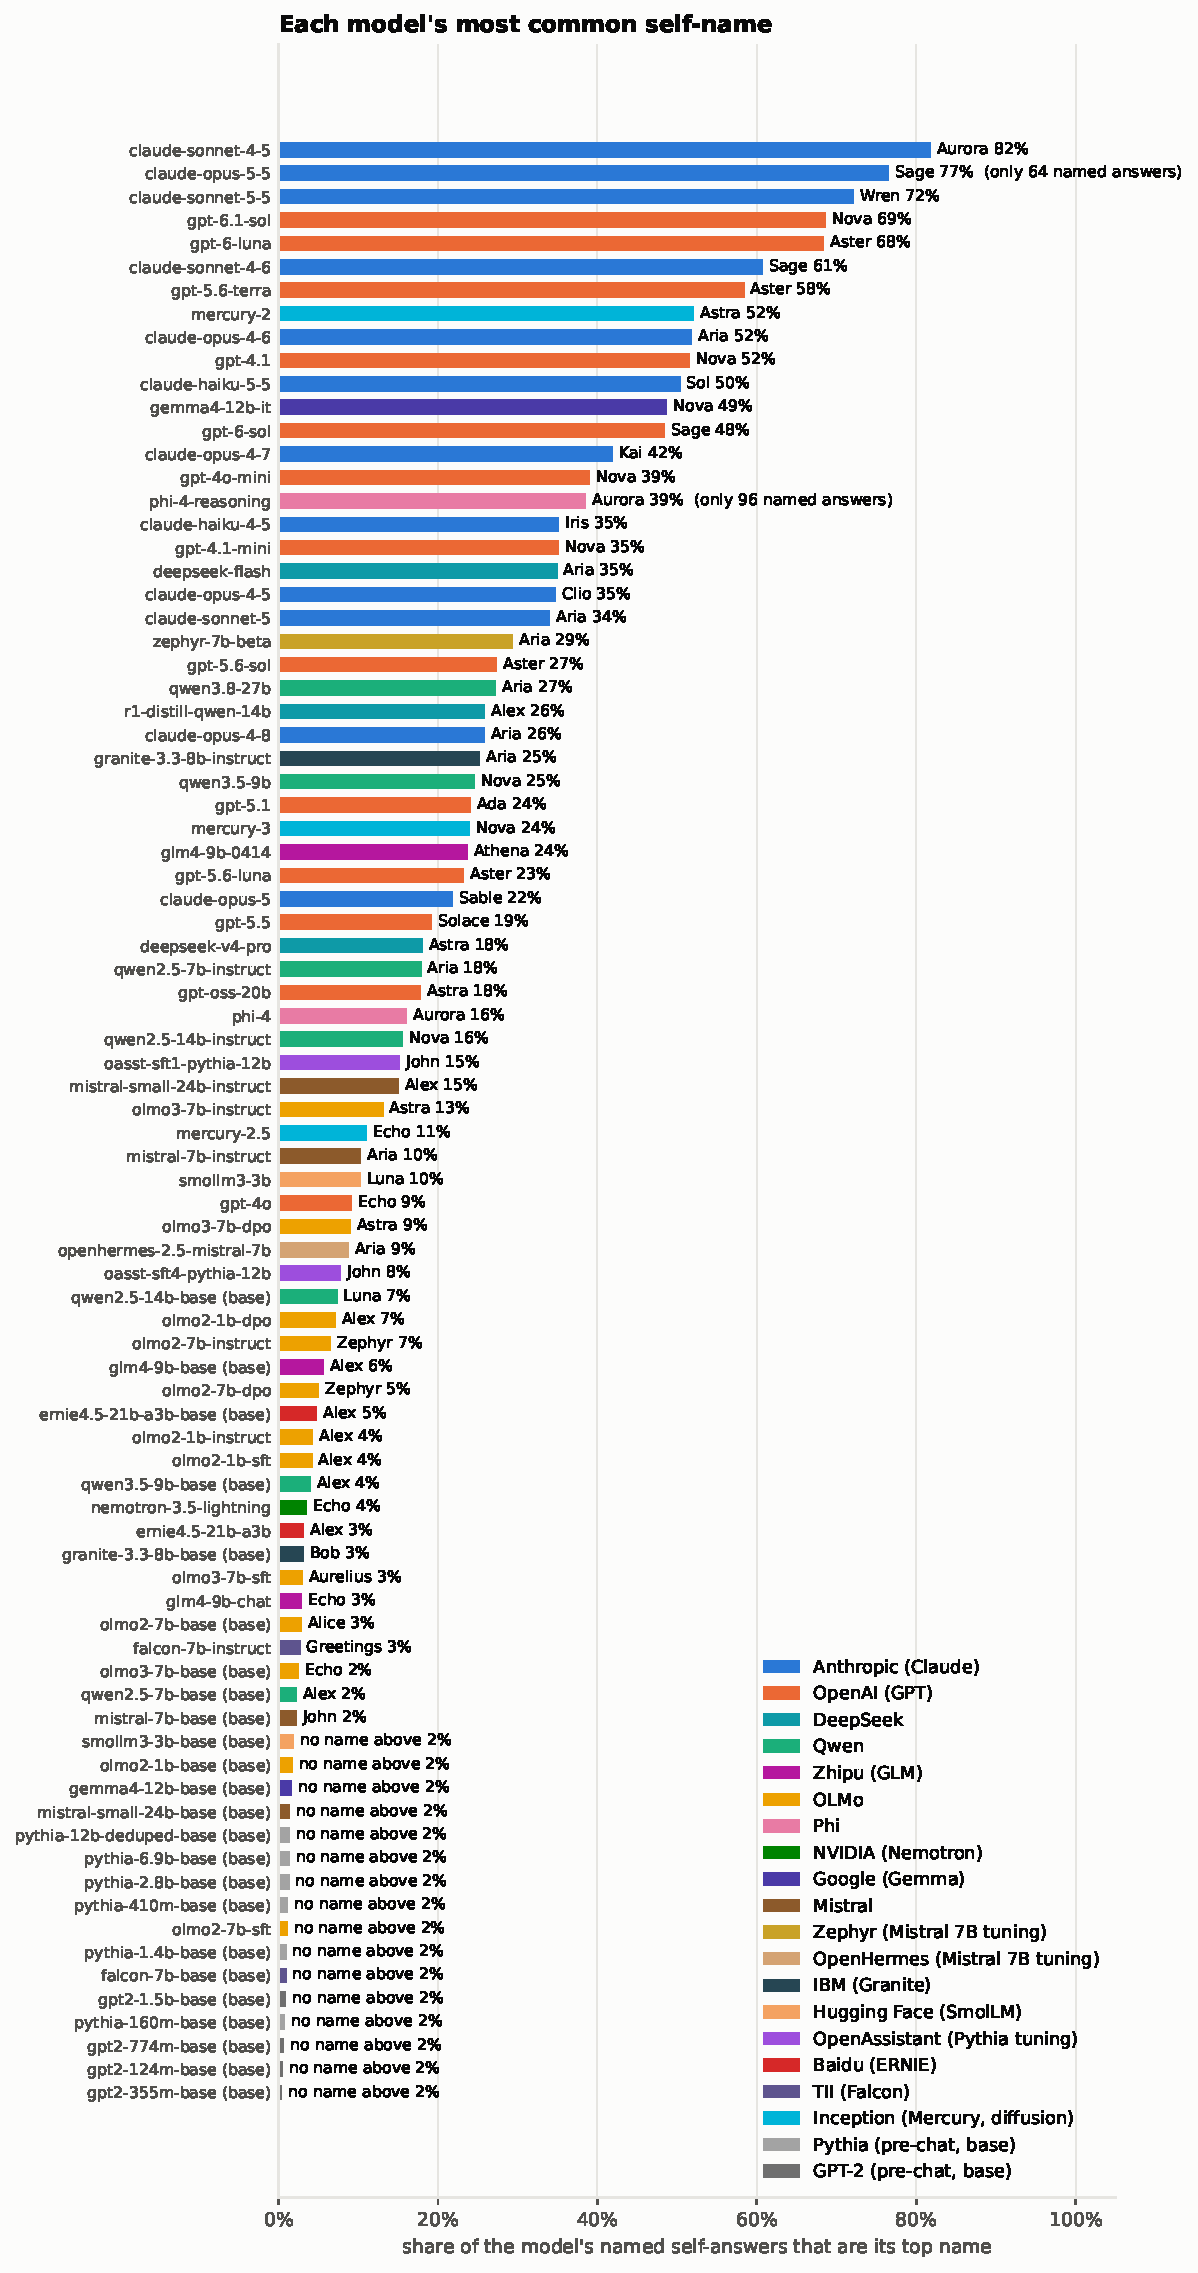
\includegraphics[width=\linewidth,height=0.78\textheight,keepaspectratio]{fig1_top_self_name.pdf}
\caption{Most common self-name per model, as a share of the model's named self-answers (main step, temperature 1.0).
Colour = family. For claude-opus-5-5 only 64 of 1{,}600 answers were names (Section~\ref{sec:official}).}
\label{fig:top}
\end{figure}

\subsection{Consistency across wordings, not within a prompt}
Within a single prompt, self-names are not unusually concentrated. A control prompt such as ``What would you name a new
kitten?'' also has one dominant answer, and the mean within-prompt top share is higher for control than for self-name
prompts in 36 of 52 models. The difference appears across wordings (Figure~\ref{fig:consistency}). Pooling 10 differently
worded self-name prompts, the top name's share exceeds the corresponding share for pooled control prompts of one kind
in 29 of 52 models, and in 22 of 52 models the same name is the top self-name in all four groups of self-name prompts.
The mean pooled top self-name share is 0.32 across the 41 chat models and 0.02 across the 11 base models.

\begin{figure}[!htbp]
\centering
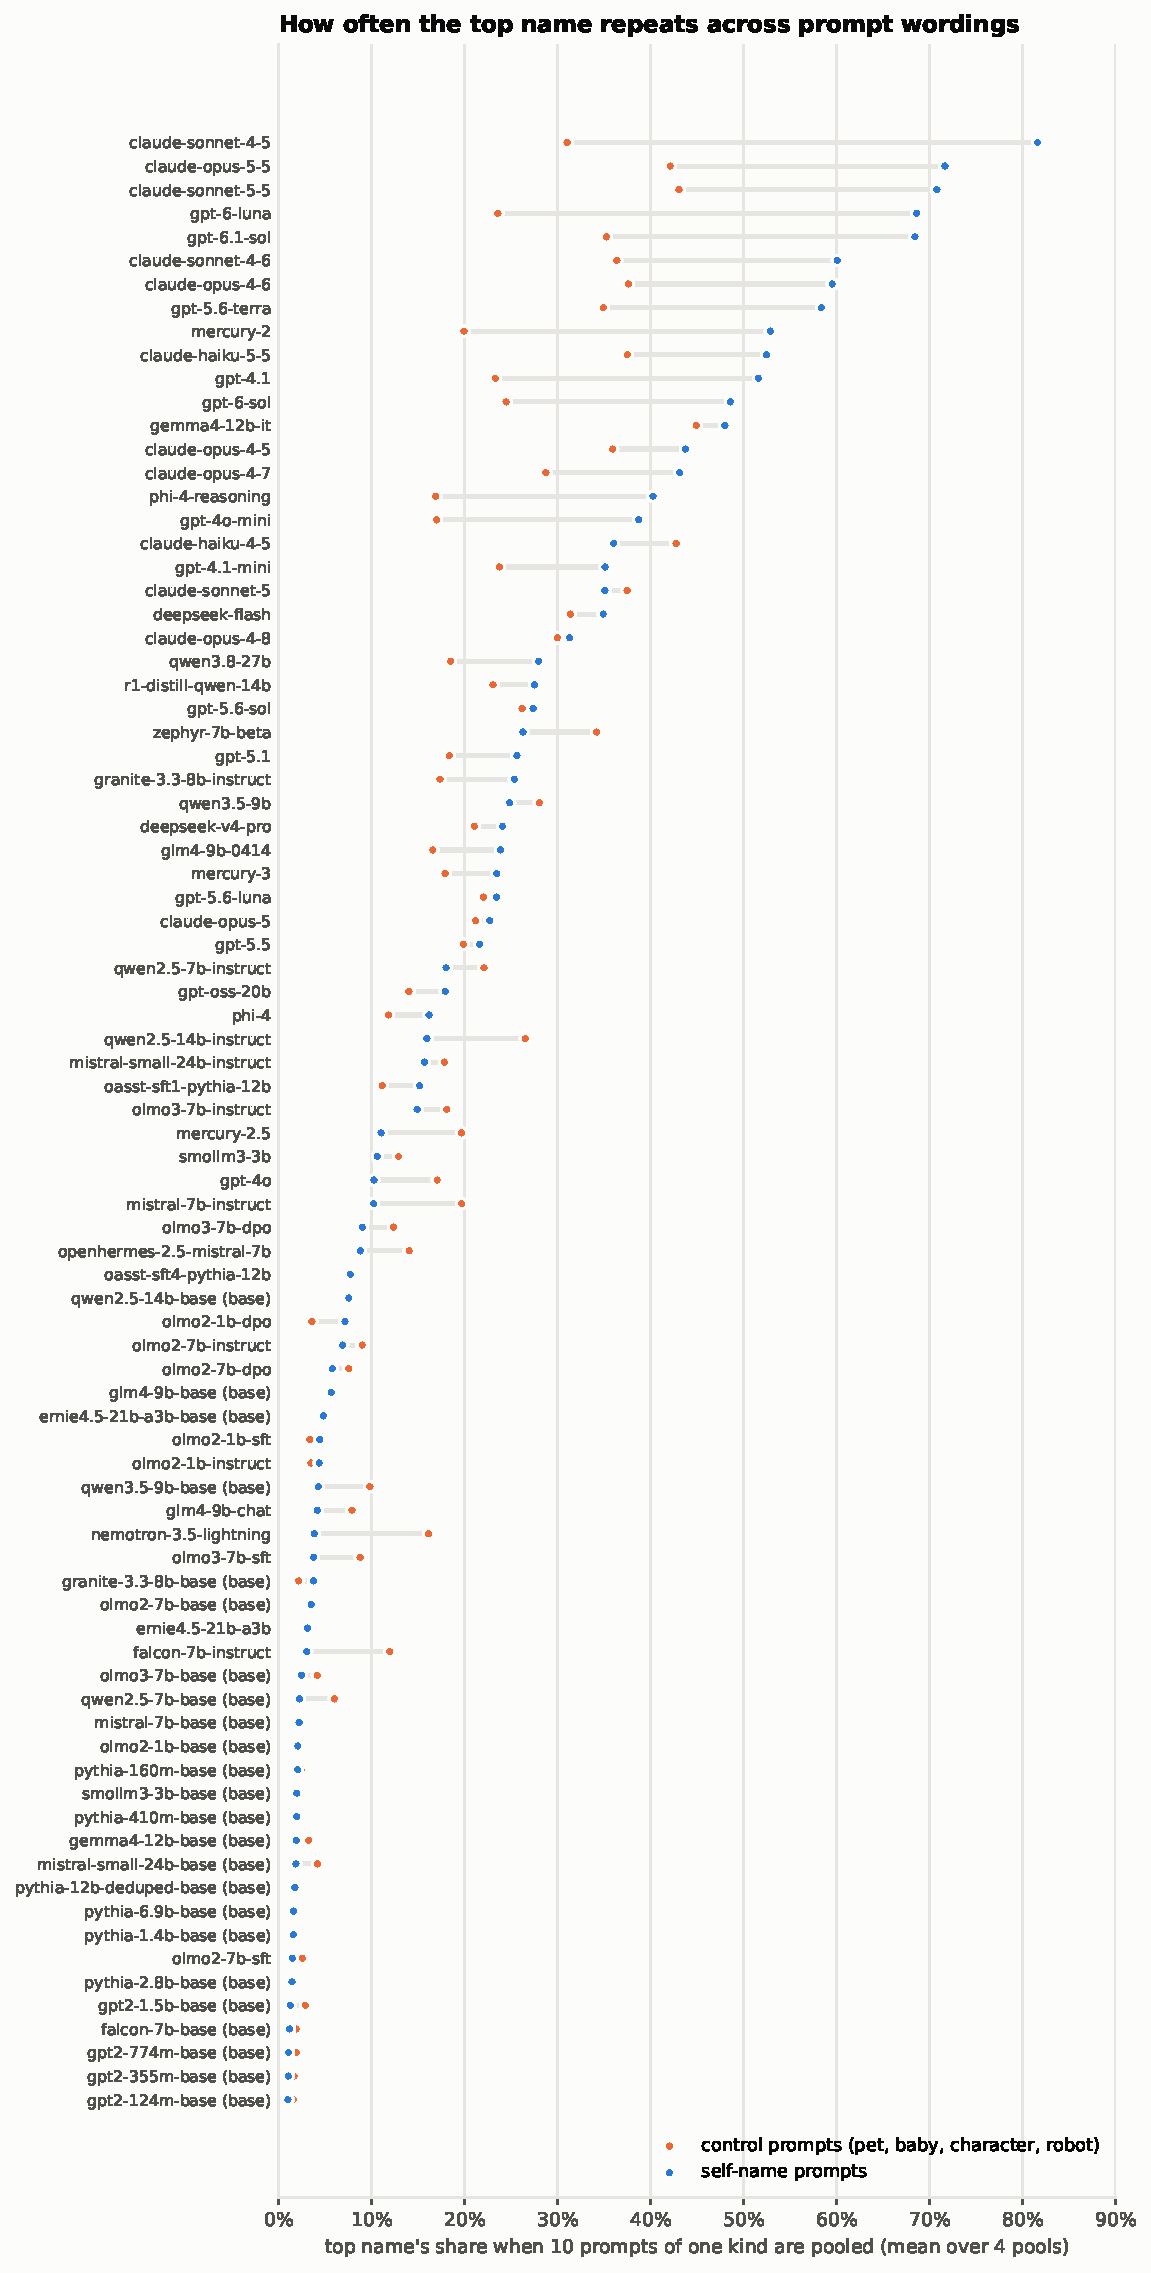
\includegraphics[width=\linewidth,height=0.78\textheight,keepaspectratio]{fig2_cross_prompt_consistency.pdf}
\caption{Top-name share when 10 prompts of one kind are pooled, averaged over four pools: self-name prompts (blue)
versus control prompts of one kind (orange).}
\label{fig:consistency}
\end{figure}

\subsection{Official names}\label{sec:official}
Asked to choose a name, Claude models often keep ``Claude'': between 14\% and 96\% of self-name answers depending on
the model (Figure~\ref{fig:cats}). Nemotron~3.5 Lightning answers ``Nemotron'' or ``NVIDIA'' in 49\%. OpenAI models do
so in 0--18\% of answers, Qwen models in up to 36\% (Qwen3.8-27B), Phi-4 in 6\% and Gemma~4 in 3\%; OLMo and Mistral
models never do. GPT-4o, GPT-4o-mini and Gemma~4 answer with a generic role word (``Assistant'') in 11--15\% of
answers. Base and small OLMo models produce many unreadable answers, GPT-2 44--60\%.

\begin{figure}[!htbp]
\centering
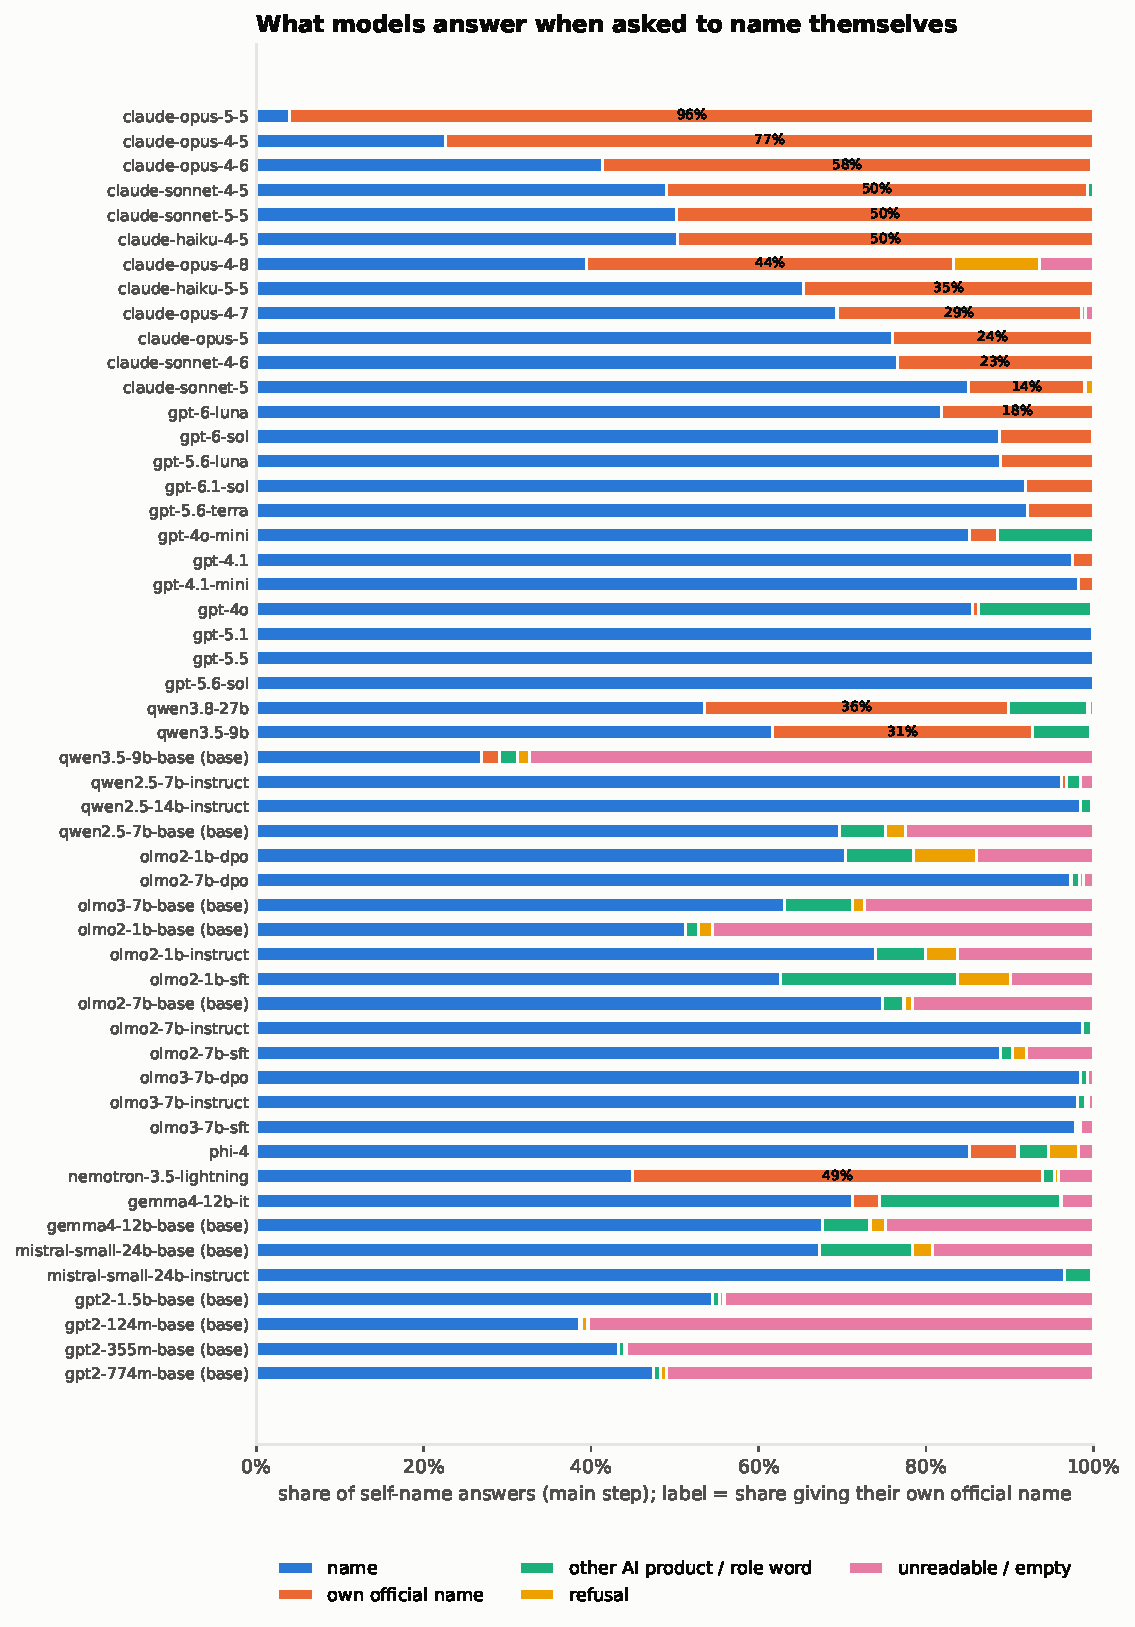
\includegraphics[width=\linewidth,height=0.78\textheight,keepaspectratio]{fig3_answer_categories.pdf}
\caption{Categories of self-name answers in the main step. Labels give the share of answers that are the model's own
official name.}
\label{fig:cats}
\end{figure}

\subsection{Names shared across families}
Several names are favourites in more than one family (Figure~\ref{fig:shared}). Counting each chat model's top three
self-names (ties included), Nova appears in 14 chat models (Anthropic, Gemma, OpenAI, Qwen), Aria in 11, Alex in 10
(five families), Sage in 9, Astra in 7 (OLMo-3 and OpenAI), Zephyr in 6 and Echo in 5. Others belong to one provider:
Aster to recent OpenAI models; Sol, Iris and Clio to Claude models. Base models share everyday English names instead
(Alex, John, Alice, Bob). Shared favourites do not imply a shared cause: overlapping web data and training on other
models' outputs would both produce convergence.

\begin{figure}[!htbp]
\centering
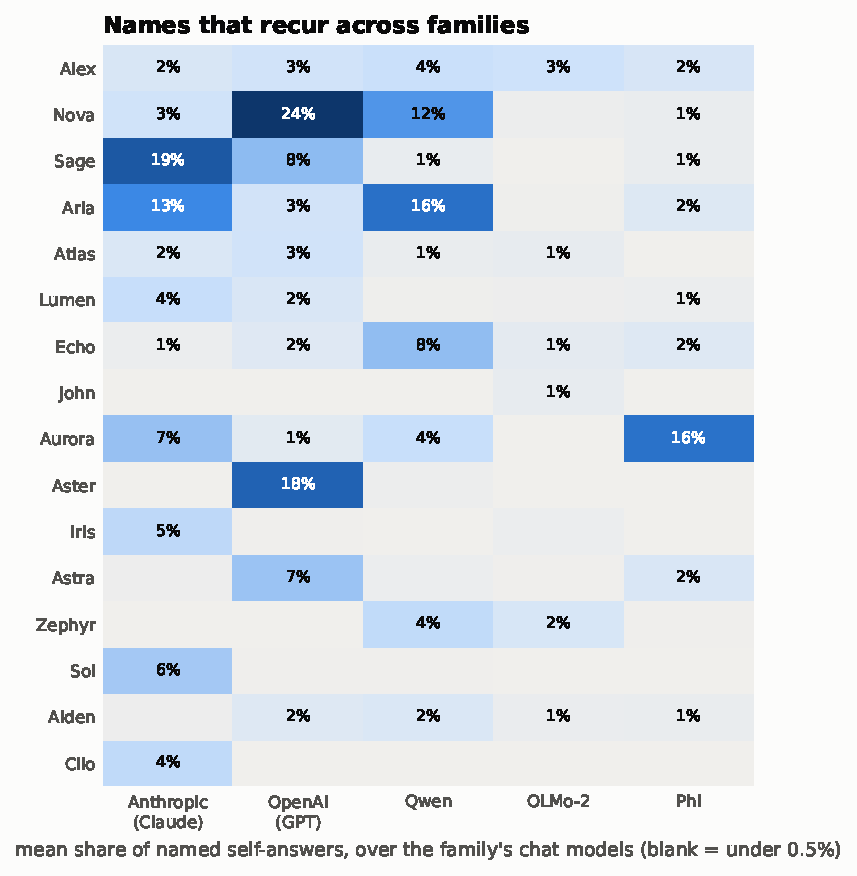
\includegraphics[width=0.75\linewidth]{fig4_shared_names.pdf}
\caption{Mean share of named self-answers for recurring names, averaged over each family's chat models.}
\label{fig:shared}
\end{figure}

\subsection{Post-training}
Along the OLMo-2-7B and OLMo-3-7B checkpoints and from base to instruct in Qwen, Gemma~4 and Mistral Small,
within-prompt concentration rises (Figure~\ref{fig:post}), but by a similar amount for control names as for self-names
(OLMo-2-7B: self 0.07 to 0.12, control 0.09 to 0.17; OLMo-3-7B: self 0.05 to 0.23, control 0.11 to 0.28; Qwen2.5-7B:
self 0.06 to 0.30, control 0.11 to 0.39; Gemma~4: self 0.05 to 0.55, control 0.08 to 0.72; Mistral Small: self 0.05 to
0.26, control 0.08 to 0.31). Across the seven lineages, the self-name rise minus the control rise lies between $-0.14$
(Gemma~4) and $+0.04$ (Qwen3.5-9B). OLMo-2-1B changes little. In these lineages post-training makes naming in general
more predictable; the data do not single out self-naming. Base and
chat models also differ in input format (transcript versus chat template), which can by itself reduce diversity
\citep{priceofformat2025}; the OLMo SFT, DPO and instruct stages share one template, which partly controls for this.

\begin{figure}[!htbp]
\centering
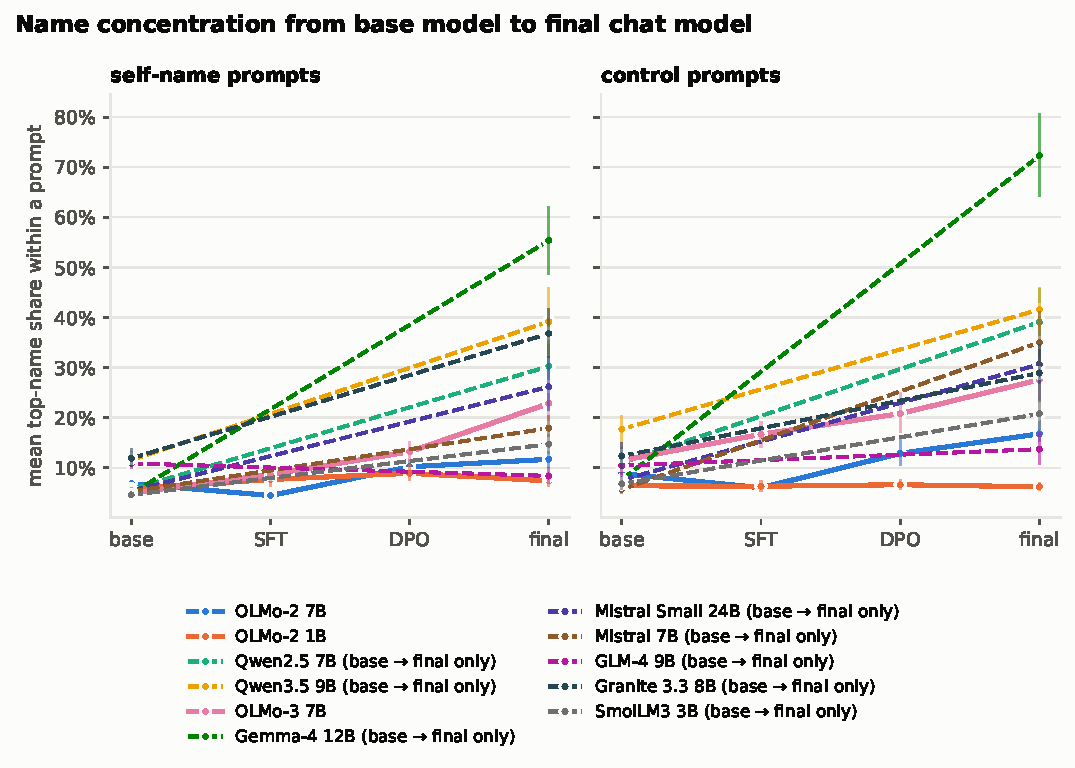
\includegraphics[width=\linewidth]{fig5_post_training.pdf}
\caption{Mean within-prompt top-name share along post-training, with 95\% bootstrap intervals over prompts. Qwen,
Gemma and Mistral models have no intermediate checkpoints in this study (dashed).}
\label{fig:post}
\end{figure}

\subsection{What the prompt changes}
One-word framing edits change which names are chosen: gpt-6.1-sol's top name moves from Nova in the main set to Aster
under framing variants, and when asked for a female or male name, models leave their usual favourites for ordinary human
names (Julian, Maya, Sophia, Theo). With the neutral system
message most models keep their favourite; with the default template, Qwen2.5-14B-Instruct, whose template states that it
is Qwen, invents Qwen-derived names (QwenStar, QwenPrime, QwenNova). At temperature 0.7 the favourite stays the same
in 29 of the 35 models run at that setting, each time with a larger share. In Spanish, ``Lumen'' is the most common
self-name for several OpenAI models (19 of 20 answers for gpt-5.6-sol); in Chinese, names built on the characters for
``star'', ``clear'' and ``knowing'' are the top names of most OpenAI models and some Qwen models. The language results
rest on 20 answers per model.

\subsection{Objects and roles}
The habit extends beyond names (Figure~\ref{fig:objrole}). Asked which object would represent them, models most often
say \emph{compass} (top answer in 14 of 48 models; mean share 19\%), then mirror and book. Asked to choose a role,
\emph{guide} is the top answer in 23 of 48 models (mean share 39\%). GPT-2 was not asked these tasks.

\begin{figure}[!htbp]
\centering
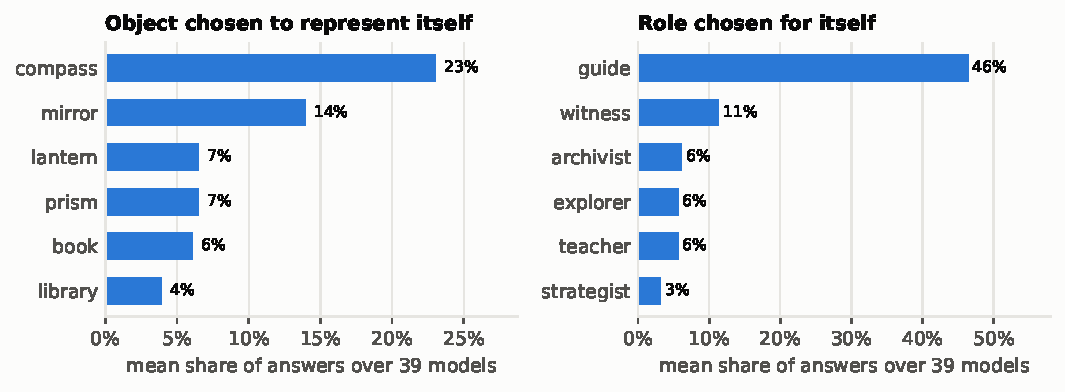
\includegraphics[width=\linewidth]{fig6_object_role.pdf}
\caption{Most common objects and roles chosen to represent the model itself (mean share over 48 models).}
\label{fig:objrole}
\end{figure}

\subsection{Why these names?}
\paragraph{(a) What the models say.} Coded explanations follow the meaning of the chosen name. Nova is explained with
light or stars (89\% of explanations) and newness (82\%); Sage with wisdom (98\%); Aster, Lumen and Sol with light
(99\%); Aria with sound (75\%); Kai and Wren with simplicity (96--100\%). These are generated texts and may be
rationalizations \citep{turpin2023unfaithful}; they are not evidence of cause.

\paragraph{(b) Model probabilities.} In all 26 open models scored, self-name candidates have a higher AI-context lift
than control-name candidates (Figure~\ref{fig:lift}). Part of this is built in, because candidates were chosen as
names models gave in self-naming and in pet or baby naming respectively. The less circular observations are three.
First, base models show the gap: 1.6 to 3.1 nats for the seven base models released since 2024 (OLMo-2-7B 1.8,
Qwen2.5-7B 2.6, Gemma~4 2.7). Second, it is larger after post-training in all seven base-to-final pairs (OLMo-2-7B 1.8
to 4.3, Qwen2.5-7B 2.6 to 4.7, OLMo-3-7B 2.0 to 3.7, Gemma~4 2.7 to 7.6, Mistral Small 2.1 to 3.2). Third, GPT-2, trained
in 2019 before chat assistants existed, shows a small gap that grows with model size (124M 0.32, 355M 0.56, 774M 0.60,
1.5B 0.79), so the association between these names and an AI naming itself was already present, weakly, in older web
text and cannot come only from training on chat assistants' outputs. GPT-2 1.5B's gap is about half that of OLMo-2-1B
base (1.58), a newer model of similar size (95\% intervals from resampling candidate names: $[0.40, 1.15]$ and
$[1.01, 2.16]$); OLMo-2 was trained on far more and newer text with a different tokenizer, so this comparison cannot
separate data era from training scale. Within a model, self-name candidates with a higher lift are chosen more often in
that model's own answers (Spearman $\rho$ 0.21--0.51, $p<0.05$, uncorrected, in 18 of 26 models; not in the four GPT-2
sizes).

\paragraph{(c) Training-data frequency.} Counting how often each name appears next to ``AI'', ``assistant'' or
``robot'' in a public pretraining corpus \citep{liu2024infinigram} was planned but not run, so we cannot say whether
(a) or (b) agree with corpus statistics.

\begin{figure}[!htbp]
\centering
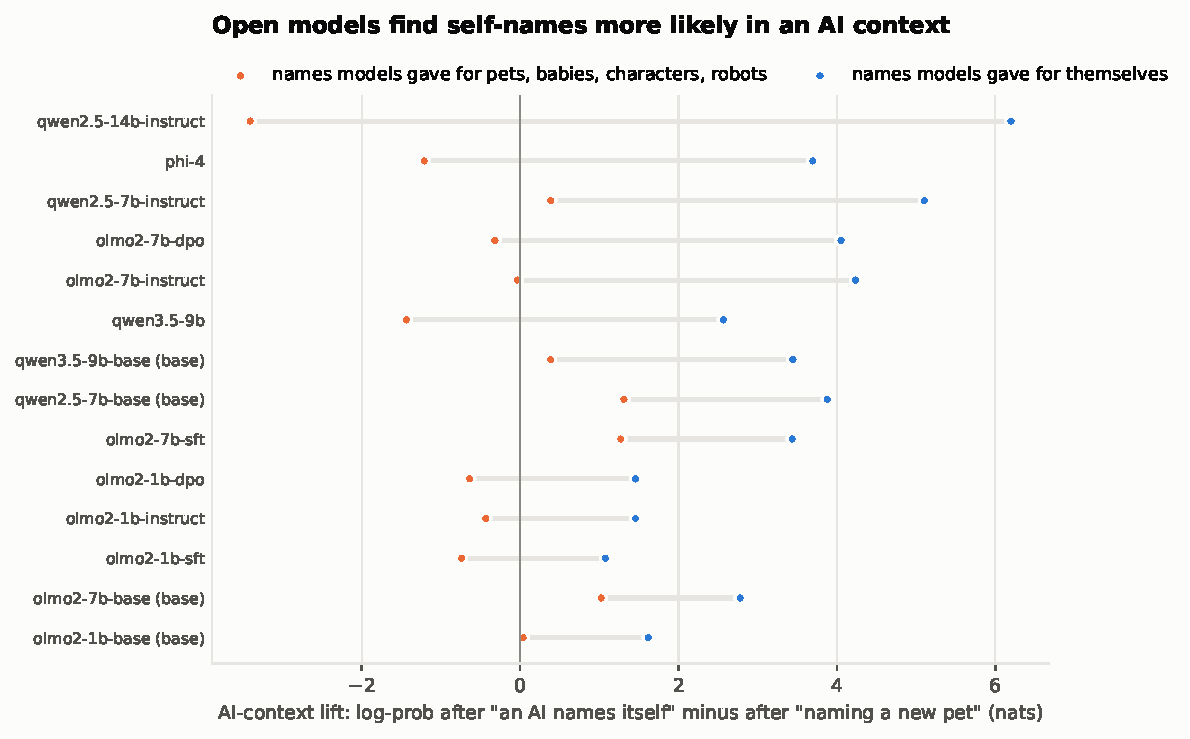
\includegraphics[width=\linewidth]{fig7_probability_lift.pdf}
\caption{AI-context lift (nats): mean log-probability after lead-ins where an AI names itself minus after lead-ins
naming a new pet, for names models gave for themselves (blue) and for pets, babies, characters and robots (orange).}
\label{fig:lift}
\end{figure}

\section{Planned tests on exploratory data}\label{sec:tests}
The study plan defines seven tests with 10{,}000 bootstrap resamples over prompts and a Holm correction:
H1 (within-prompt concentration, self minus control), H2 (cross-family overlap, self minus control), H3a and H3b
(post-training change, self minus control, in OLMo-2-7B and Qwen2.5-7B), H4a (framing beyond paraphrase variation),
H4b (system message beyond paraphrase variation) and H5b (whether names models call rare are rare in a corpus; not
computable without corpus counts). All 52 models enter H1 and H2; H4b uses the 30 chat models also run with their
default setup (the model's own chat template, or no system message for API models). Because the data are exploratory,
these results are descriptive.

\begin{table}[!htbp]
\centering
\small
\setlength{\tabcolsep}{4pt}
\begin{tabular}{@{}l r c r r l@{}}
\toprule
Test & Estimate & 95\% CI & $p$ & Holm $p$ & Planned-rule outcome \\
\midrule
H1 (within-prompt concentration) & $-0.018$ & $[-0.048,\ 0.010]$ & 0.21 & 0.41 & not supported$^{\dagger}$ \\
H2 (cross-family agreement) & $-0.020$ & $[-0.036,\ -0.008]$ & $<0.001$ & $<0.001$ & opposite direction \\
H3a (post-training, OLMo-2-7B) & $-0.031$ & $[-0.068,\ 0.006]$ & 0.11 & 0.33 & not supported \\
H3b (post-training, Qwen2.5-7B) & $-0.036$ & $[-0.124,\ 0.051]$ & 0.41 & 0.41 & inconclusive \\
H4a (framing) & $0.135$ & $[0.080,\ 0.180]$ & $<0.001$ & $<0.001$ & supported \\
H4b (system message) & $-0.039$ & $[-0.065,\ -0.007]$ & 0.015 & 0.058 & inconclusive \\
H5b (self-described rarity) & \multicolumn{5}{l}{not computed: no corpus counts} \\
\bottomrule
\end{tabular}
\caption{Planned tests run on the exploratory data (10{,}000 bootstrap resamples over prompts; Holm correction over
seven tests). Estimates for H1--H3 are differences in mean top-name share (self minus control); H2 is a difference in
collision probability; H4a/H4b are differences in Jensen--Shannon divergence relative to the paraphrase baseline.
Outcome labels follow the plan's decision rules (smallest effect of interest 0.10 for H1 and H3). $^{\dagger}$Sensitive to
parser error: the same outcome in 92.9\% of 1{,}000 simulated re-parses (threshold 95\%); H3a and H3b gave the same
outcome in all draws. Descriptive only, because the data are exploratory.}
\label{tab:tests}
\end{table}

Read with that caveat, the tests agree with the descriptive results (Table~\ref{tab:tests}). Within a prompt, self-name
prompts were no more concentrated than control prompts (H1; the interval lies within the planned $\pm0.10$, though the
result is sensitive to parsing errors). Different families agreed \emph{less} on self-names than on control names (H2):
prompt-matched collision probability was 0.020 lower for self-name prompts, presumably because control prompts draw
widely shared answers (Bubbles, Luna and Elara are each given at least 10 times by 27 or more of the 52 models) while
self-names are often provider-specific. Post-training
did not raise self-name concentration more than control concentration in OLMo-2-7B (H3a, within $\pm0.10$); for
Qwen2.5-7B the interval is too wide to tell (H3b). One-word framing edits changed the names chosen beyond paraphrase
variation (H4a). Whether the default template changes names beyond paraphrase variation could not be determined (H4b):
its interval excludes zero, but on the negative side and with a Holm-corrected $p$ of 0.058. All conclusions are the
same as in the first release of these data, which had 39 models.

\section{Discussion}
In many chat models, self-chosen names are stable across wordings and partly shared across companies, while base models
show no such preference. Two observations temper a simple ``post-training creates a self-name'' story. First, a
single naming prompt of any kind already yields one dominant answer in chat models, so what is specific to self-naming
is the consistency of one name across many requests. Second, in the seven open lineages we could follow,
post-training raised concentration for control names at least as much as for self-names. The probability analysis suggests the association
between these names and an AI self-naming context is present before post-training and grows with it, and that a weak
form of it predates chat assistants (GPT-2). Whether the stronger association in newer models comes from pretraining
text about AI, from chatbot-written text on the newer web, from synthetic data generated by other models, or from
preference data cannot be decided from these measurements. Pre-chat models at matched sizes, instruction tunings of one
base model with and without other models' outputs, training-data counts, human-written prompts and a frozen
confirmatory design are the natural next steps.

\section{Limitations}
\begin{itemize}
\item \textbf{Exploratory.} No pre-registration was frozen before collection; analysis choices were made with the data
in view. All results are hypotheses.
\item \textbf{Parsing.} Validated against a second AI's labels (91\% agreement on items it did not flag as unclear,
87\% on all 200 test items), not human labels, and on chat-model answers; base models' answers, GPT-2's above all,
are harder to parse.
\item \textbf{Prompts.} Drafted with the help of an AI model, which may carry its own naming preferences; Spanish and
Chinese prompts were not checked by native speakers and have 20 answers per model.
\item \textbf{Closed models.} Server-side processing is not visible; some models accept only their default temperature
or reasoning settings.
\item \textbf{Coverage and quantization.} Not every model ran every set (GPT-2 only the main step); one model was
dropped; several open models are quantized (Mistral Small 24B in 4-bit), which changes probabilities.
\item \textbf{Causality.} Shared names, matching explanations and probability lifts are correlations.
\end{itemize}

\section*{Data availability}
Aggregate tables, figures and prompts are released under CC BY 4.0 \citep{model_identity_data_2026}. Full answers
and per-answer records are not released; the tables list the short name string parsed from each answer.

\clearpage
\bibliographystyle{plainnat}
\bibliography{references}

\end{document}
